\chapter{Przetwarzanie danych masowych na platformach\\równoległych} \label{chap.big-data-processing}

\section{Podstawowe definicje}
\subsection{Big data}
Definicja pojęcia Big data (dane masowe) jest dosyć rozległa i jednocześnie rozmyta. Świat informatyki kieruje się ku definicji iż big data występuje wszędzie tam gdzie wymagane jest przetworzenie wielkiej ilości danych. Jednocześnie nie jest zdefiniowana jednostka oraz jej wielkość od której możemy mówić o big data. Firma SAS opisuje termin big data jako: \newline \textit{"Big data is 
a  popular  term  used  to  describe  the  exponential  growth,  
availability  and  use  of  information,  both  structured  and  
unstructured"}. \newline Z kolei firma IBM big data definiuje jako: \textit{“Data, 
coming  from  everywhere;  sensors  used  to  gather  climate  
information,  posts  to  social  media  sites,  digital  pictures  
and  videos,  purchase  transaction  record,  and  cell  phone  
GPS signal to name a few”}.\cite{big_data_concept} Bazując na powyższym źródle możemy stwierdzić iż big data to zwyżkujący trend, który wskazuje na błyskawiczny przyrost danych pochodzących z różnych źródeł w krótkim okresie czasu. Jednocześnie wskazujący na znaczącą wartość danych po ich późniejszym przetworzeniu. Dla końcowego użytkownika, można uprościć, że big data to niedefiniowany zbiór różnych danych zawierający wartościowe informacje w nieustrukturyzowanej formie.
\subsection{4V}
W związku z mocno niedoprecyzowanym pojęciem big data publikacje naukowe definiują wymiary, które określają właściwości danych masowych.\cite{big_data_great_services} Kategorie te określa się pojęciem \textbf{4V}. Jest to skrót opisujący cztery wartości:
\begin{itemize}
	\item Objętość (Volume)
	\item Różnorodność (Variety)
	\item Prędkość (Velocity)
	\item Wiarygodność (Veracity)
\end{itemize}
Objętość wynika z samego rozmiaru danych. W założeniach są to rozmiary wielkie lecz nie można zdefiować dokładnej wielkości oraz jednostki od której można stwierdzić iż dany zbiór danych już się kwalifikuje do zbioru big data. Brak jasno określonej wielkości ma sens ze względu na założenie, że zbiór big data jest nieskończony i stale rosnący. W związku z czym wielkość wymiaru ulega ciągłej zmianie.\newline
Różnorodność zakłada nieustrukturyzowanie danych. Użytkownik działający w środowisku big data jest nastawiony na dużą ilość danych, jednocześnie jest przygotowany na zorganizowanie ich samodzielnie w logiczną strukturę danych. Różnorodność to również wiele formatów danych: tekst, multimedia, grafika, dzwięk.\newline
Prędkość mówi o tempie generacji danych, które są tworzone przez wiele różnych podmiotów: ludzi, maszyn, wszelkiego rodzaju czujników. Jest to również pośrednie do samej techniki przetwarzania danych \textbf{streaming} \ref{streaming_subsection}.\newline
Wiarygodność to nic innego jak stopień poprawności danych. Wiele danych może być wygenerowanych błędnie, mogą być niekompletne, uszkodzone. Użytkownik systemu danych masowych musi samemu zdefiniować stopień do którego ufa danym na podstawie których dokonuje analizy.\newline
Ostatnim wymiarem, który nie podlega bezpośrednio terminowi 4V jest wartość (value). Jest to nie jako wypadkowa tego terminu - jaką wartość końcową stanowią dla użytkownika końcowego dane masowe. Czy wynik ich analizy przynosi realną wartość, czy koszty poniesione w stosunku do pozyskania oraz przetworzenia danych były niższe niż warość uzyskanych rezultatów?
\subsection{Klaster komputerowy}
Klaster komputerowy to najbardziej podstawowa jednostka obliczeniowa jeżeli chodzi o systemy rozproszone. Jest to zestaw połączonych między sobą samodzielnych komputerów, które mogą wymieniać wzajemnie informacji. Połączenie komputerowe opiera się o łącze o wysokiej przepustowości np. Ethernet, co gwarantuje obniżenie kosztów dystrybucji danych. Każda maszyna włączona do klastra posiada własny procesor obliczeniowy, pamięć RAM\footnote{Random access memory}, przestrzeń dyskową. Jednocześnie z punktu widzenia końcowego użytkownika, klaster posiada jeden punkt wejściowy dla obliczeń (API)\footnote{Application programmer interface}. Dzięki temu końcowy użytkownik nie jest zmuszony do zarządzania zasobami wewnętrznymi klastra i obsługuje tylko jedno źródło wprowadzania danych.\cite{cluster_grid_cloud} 
\newline Główną zaletą klastrów obliczeniowych jest wysoka dostępność. Z racji swojej rozproszonej architektury, która udostępnia łatwą skalowalność wszerz, możliwe jest dokładanie kolejnych komputerów by zwiększyć moc obliczeniową. Jednocześnie gdy moc obliczeniowa w danej jednostce czasu nie jest wymagana, komputery mogą zostać dynamicznie oddelegowane w stan uśpienia lub do innych zadań. Takie rozwiązanie jest bardzo elastyczne ze względu na potrzeby końcowego użytkownika. Dodatkowym aspektem jest stabilność klastrów. Gdy jakiś z elementów klastra ulega awarii, system monitoringu może łatwo wyszukać wadliwą jednostkę, usunąć ją z klastra i dołożyć nową, sprawną. Takie działanie pozwala użytkownikowi na korzystaniu z bardzo stabilnego rozwiązania, bez konieczności redukcji mocy obliczeniowej.\cite{cluster_grid_cloud_detailed_comparison}
\subsection{Obliczenia równoległe}
Obliczenia równoległe to rozdzielanie poszególnych zadań dla niezależnych procesów, które z definicji posiadają osobną przestrzeń pamięci. Takie podejście jest wykorzystywane podczas przetwarzania danych masowych w klastrze komputerowym (każda maszyna jest oddzielnym procesem). Dzięki temu większość operacji jest wykonwana niezależnie co pozwala na zaoszczędzenie czasu w stosunku do obliczeń wielowątkowych, które zakładają zależność między sobą. Prof. Charles E. Leiserson wykładający na uczelni MIT\footnote{Massachusetts Institute of Technology} definuje obliczenia równoległe jako:
\newline \textit{A form of computing in which computations are broken into many pieces that are executed simultaneously}.\cite{mit_presentation}
\subsection{Obliczenia wielowątkowe}
Obliczenia wielowątkowe to rozdzielenie poszególnych zadań między wątki aplikacji, które współdzielą przestrzeń adresową między sobą. W kontekscie obliczeń w klastrze nie mają aż tak dużego znaczenia, gdyż nie gwarantują wysokiego poziomu niezależności. Wielowątkowość jest definiowana przez Prof. Charles E. Leiserson'a następująco: 
\newline \textit{A form of computing in which computations are designed as collections of interacting processes.}\cite{mit_presentation}
\section{Dostępne oprogramownie na rynku danych masowych}
Na rynku danych masowych jest mnóstwo narzędzi, które wspierają przetwarzanie danych o dużych objętościach. Możemy podzielić je na następuje kategorie:
\begin{itemize}
	\item Eksploracja danych (Data discovery)
	\item Analityka biznesowa (Business Intelligence)
	\item Analiza bazodanowa (In-database analytics)
	\item Wysoko dostępne rozproszone zorientowane obiektowo platformy\footnote{High-availability distributed	object oriented platform - Hadoop}
	\item Zarządzanie decyzją (Decision management)    
\end{itemize}
Narzędzia z kategorii \textit{eksploracja danych} służą głównie do wydobywania informacji ze zbiorów danych o dużej objętości na podstawie danych wejściowych. Ich format jest dowolny. Często narzędzia tego rodzaju łączy się z narzędziami z dziedziny \textit{analityki biznesowej}. Dzięki takiemu podejściu można dokonywać analiz, raportów bądź pomiarów wydajności. \textit{Analiza bazodanowa} to operowanie na danych masowych po stronie bazy danych. Ta kategoria zakłada iż logika analizy danych jest zarazem częścią źródła danych. Często wykorzystwana podczas próby znalezienia relacji między danymi. \textit{Zarządzanie decyzją} - narzędzia wspomagające, bądź podejmujące decyzje na podstawie już dokonanej analizy danych. \textit{Wysoko dostępne rozproszone zorientowane obiektowo platformy} są szczególnie użyteczne podczas wstępnego przetwarzania danych. Jest to szczególnie ważne by pierwotny zbiór danych był okrojony i jednocześnie zawierał jak najwięcej wartościowych informacji. Takie podejście oszczędza czas oraz zasoby podczas bardziej złożonej analizy danych.\cite{big_data_tools}
\newline Zauważalne jest, że dane masowe mogą być przetwarzane w różnoraki sposób. Metoda analizy powinna być dobrana w zależności od potrzeb i dostępnych zasobów obliczeniowych. Ze względu na zwyżkującą popularność nowego narzędzia w kategorii \textit{Hadoop} - Apache Spark w konkteście tej pracy magisterskiej dokonane jest jego porównanie z Apache Hadoop.\cite{databricks_survey}  
\section{Paradygmat Map Reduce}
Paradygmat Map Reduce to główne założenie rozproszonego przetwarzania danych. Pomysł zrodził się w firmie Google. Internetowy gigant potrzebował łątwo skalującego się rozwiązania, które można by było zastosować do indeksowania danych, które obsługiwała wyszukiwarka. Map reduce dzięki swojej łatwej rozszerzalności i możliwości zamiany bądz usuwania poszególnych części systemu obliczeniowego pozwolił na duże oszczędności oraz elastyczność w kwesti utrzymania systemu indeksowania. Rozszerzalność była szczególnie ważnym elementem gdyż indeksowany zbiór danych ciągle zwiększał swój zasób.
\newline
Map reduce pozwala na dzielenie dużego zbioru danych na części i wykonanie operacji na mniejszej ilości danych na danym serwerze należący do klastu komputerowego. Dzięki temu do analizy danych o dużej objętości mogą zostać zastosowane komputery o mniejszej mocy obliczeniowej, które są jednocześnie zdecydowanie tańsze w zakupie i utrzymaniu. Metoda dzieli się na dwa głowne kroki:
\begin{itemize}
	\item Map
	\item Reduce 
\end{itemize}
Krok \textbf{map} przyjmuje główną porcję danych, dzieli na mniejsze części. Następnie podzielone już porcje danych są wysyłane na poszeczególne węzły(serwery) klastra komputerowego. Krok \textbf{reduce} jest odpowiedzialny za zebranie danych poddanych obróbce przez klaster. Po dokonanym kolekcjonowaniu zwracany jest wynik analizy wielkiego zbioru danych.\cite{map_reduce_description}
\newline MR\footnote{Map Reduce} możemy zapisać funkcyjnie jako:
\begin{equation}
map(k1,v1) \to list(k2,v2)
\end{equation}
\begin{equation}
reduce(k2, list (v2)) \to list (v3)
\end{equation}
gdzie \textit{map} przyjmuje problem $k1$ z dziedziny $v1$ i zwraca listę podproblemów $k2$ z dziedziny $v2$. Następnie MR zbiera wszystkie pary z tym samym kluczem $k2$ ze wszystkich list i grupuje je razem tworząc jedną grupę dla każdego klucza. Operacja \textit{reduce} jest wykonywana równolegle ($list(v2)$) dla każdej grupy. Wynikiem jest lista wartości $v3$, która może być pusta.\cite{map_reduce_microsoft_article}
\newline Przykładowa implementacja dla zliczania ilości poszczególnych słów w danym dokumencie dla języka scala jest przedstawiona w listingu \ref{lst:scala_word_count}.
\begin{lstlisting}[language=scala, caption={Przykład "Word Count"},captionpos=b, label={lst:scala_word_count}]
//Transformacja struktury danych
val slowa = plik_wejsciowy.flatMap(linia => linia.split(" "))
// Rozdzielenie dziedziny na podproblemy
val podproblemy = words.map(slowo => (slowo, 1))
// Redukcja danych - zliczenie wystapien poszczegolnych slow
val liczba_wystapien = podproblemy.reduceByKey{case (x, y) => x + y}
\end{lstlisting}
Architektura paradygmatu MR jest przedstawiona na rysunku \ref{fig:@=map_reduce_schema}.\cite{map_reduce_figure} 
\begin{figure}
	\centering
	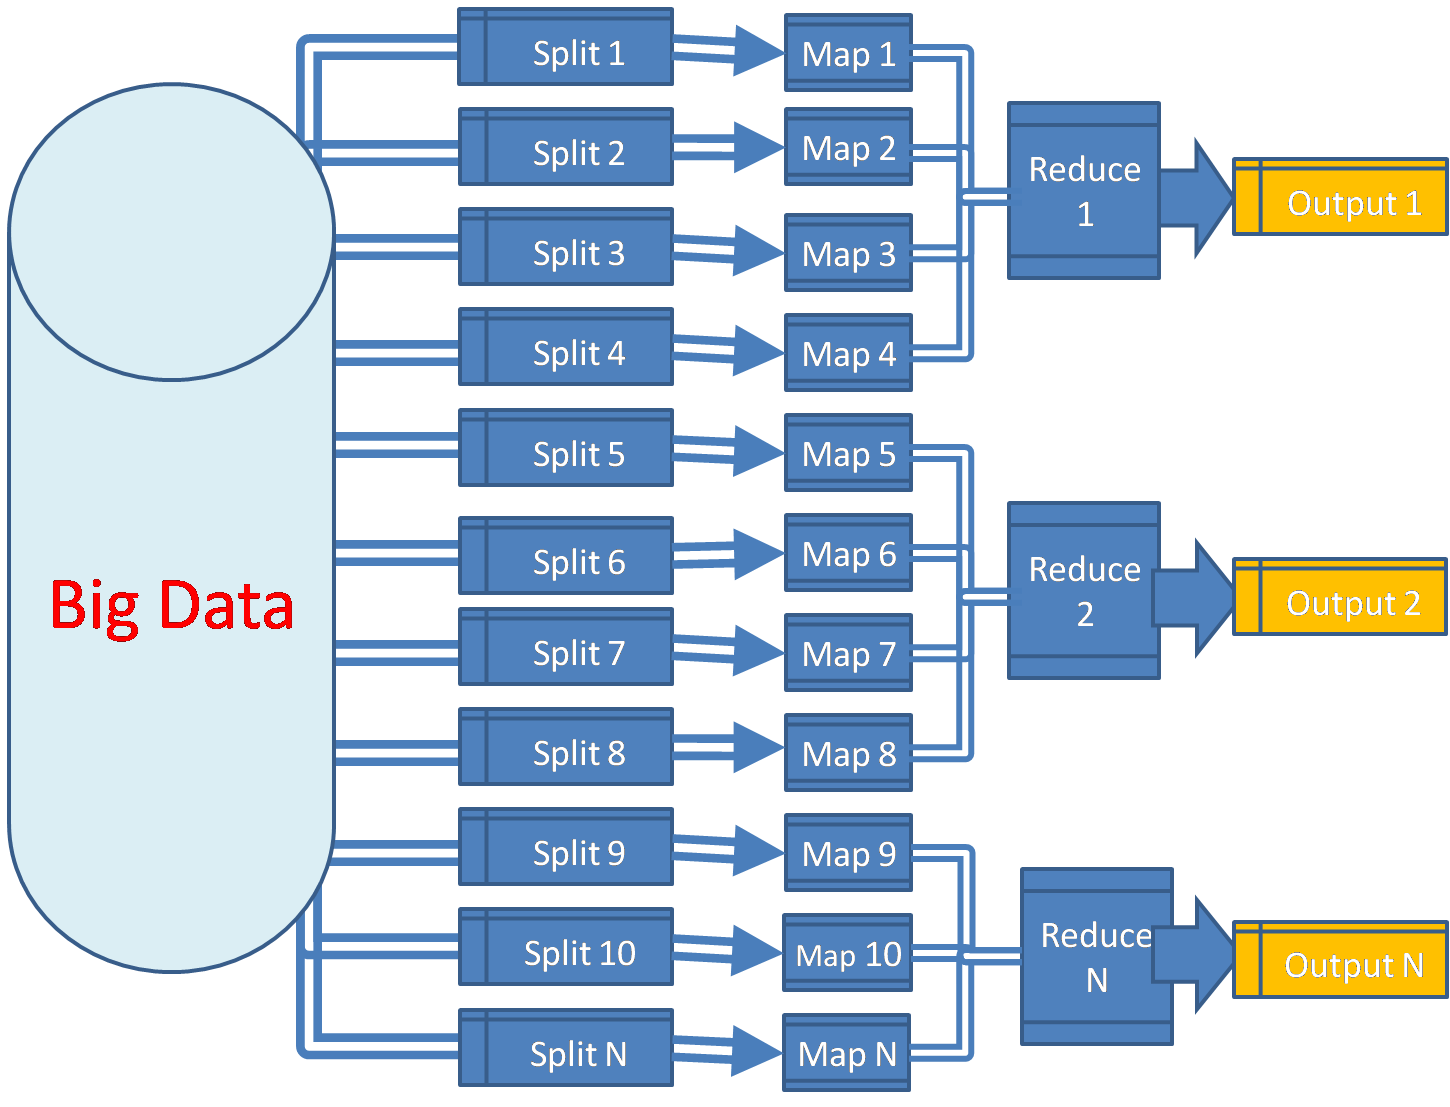
\includegraphics[scale=0.3]{map_reduce_flow.png}
	\caption{Architektura Map Reduce}
	\label{fig:@=map_reduce_schema}
\end{figure}
\subsection{Faza Shuffle w Map Reduce}
\section{Wykonywanie obliczeń przy użyciu klastrów komputerowych}
\section{Operacje - przypadki użycia w architekturze równoległej}
